\documentclass[12pt,a4paper]{article}

% Packages
\usepackage[utf8]{inputenc}
\usepackage[vietnamese]{babel}
\usepackage{geometry}
\usepackage{graphicx}
\usepackage{hyperref}
\usepackage{listings}
\usepackage{xcolor}
\usepackage{amsmath}
\usepackage{float}
\usepackage{caption}
\usepackage{subcaption}
\usepackage{enumitem}
\usepackage{fancyhdr}
\usepackage{titlesec}
\usepackage{tocloft}

% Page geometry
\geometry{
    left=3cm,
    right=2cm,
    top=2.5cm,
    bottom=2.5cm
}

% Header and footer
\pagestyle{fancy}
\fancyhf{}
\fancyhead[L]{Vending Machine System}
\fancyhead[R]{STM32 Project Report}
\fancyfoot[C]{\thepage}

% Code listing style
\lstdefinestyle{cstyle}{
    language=C,
    basicstyle=\ttfamily\small,
    keywordstyle=\color{blue}\bfseries,
    commentstyle=\color{gray}\itshape,
    stringstyle=\color{red},
    numbers=left,
    numberstyle=\tiny\color{gray},
    stepnumber=1,
    numbersep=8pt,
    backgroundcolor=\color{white},
    showspaces=false,
    showstringspaces=false,
    showtabs=false,
    frame=single,
    rulecolor=\color{black},
    tabsize=4,
    captionpos=b,
    breaklines=true,
    breakatwhitespace=false,
    escapeinside={(*@}{@*)}
}

\lstset{style=cstyle}

% Hyperref setup
\hypersetup{
    colorlinks=true,
    linkcolor=black,
    citecolor=blue,
    urlcolor=blue,
    pdftitle={Vending Machine Technical Report},
    pdfauthor={Nguyen Hung Thinh, Le The Loc, Tran Doan Hoang Lam}
}

% Title information
\title{
    \Large\textbf{TRƯỜNG ĐẠI HỌC BÁCH KHOA TP.HCM}\\
    \large Khoa Khoa học và Kỹ thuật Máy tính\\
    \vspace{0.5cm}
    \includegraphics[width=8cm]{../Pictures/hcmut.png}\\
    \rule{\textwidth}{1.5pt}\\
    \vspace{0.5cm}
    \Huge\textbf{MÁY BÁN HÀNG TỰ ĐỘNG}\\
    \Large\textbf{Báo cáo}\\
    \vspace{0.3cm}
    \Large Đồ án môn học Thiết kế Luận lý\\
    \rule{\textwidth}{1.5pt}\\
}

\author{
    \textbf{Giảng viên hướng dẫn:}\\
    Nguyễn Thành Lộc\\
    \vspace{1cm}\\
    \textbf{Nhóm tác giả:}\\
    Nguyễn Hưng Thịnh\\
    Lê Thế Lộc\\
    Trần Doãn Hoàng Lâm\\
    \vspace{3cm}
}

% Get current date in Vietnamese format automatically
\date{\today}

\begin{document}

% Title page
\maketitle
\thispagestyle{empty}

\newpage

% Table of contents
\renewcommand{\contentsname}{Mục lục}
\tableofcontents
\newpage

% Main content
\newpage
\section{Sơ lược Hệ thống}

\begin{figure}[H]
    \centering
    \includegraphics[width=0.9\textwidth]{../Pictures/architecture.png}
    \caption{Sơ đồ hệ thống}
    \label{fig:system_architecture}
\end{figure}

\subsection{Yêu cầu đặt ra}

\begin{enumerate}[label=FR\arabic*:, leftmargin=*]
    \item \textbf{Tự động ON/OFF:} Hệ thống sẽphát hiện sự hiện diện của người dùng trong phạm vi 20cm trong 3 giây liên tiếp và tự động bật nguồn
    
    \item \textbf{Duyệt Sản phẩm:} Người dùng sẽ điều hướng qua 16 sản phẩm bằng các phím Lên/Xuống
    
    \item \textbf{Thông tin Sản phẩm:} Màn hình sẽ hiển thị tên sản phẩm, số lượng có sẵn và giá bán
    
    \item \textbf{Chọn Số lượng:} Người dùng sẽ nhập số lượng từ 1-9 đơn vị, nếu có lỗi thì sẽ thông báo yêu cầu nhập lại
    
    \item \textbf{Thanh toán:} Hệ thống sẽ chấp nhận các mệnh giá (5K, 10K, 20K, 50K, 100K, 200K, 500K VND) và tính toán tiền thừa
    
    \item \textbf{Quản lý Kho hàng:} Hệ thống sẽ theo dõi mức tồn kho và không bán món hàng đã hết hàng
    
    \item \textbf{Lưu trữ Dữ liệu:} Dữ liệu kho hàng sẽ luôn được lưu lại kể cả khi mất điện
    
    \item \textbf{Quản trị:} Chế độ quản trị được bảo vệ bằng mật khẩu sẽ cho phép điều chỉnh kho hàng và giá cả
    
    \item \textbf{Lỗi:} Hệ thống sẽ xử lý các đầu vào không hợp lệ, thời gian chờ và hiển thị các thông báo lỗi thích hợp
    
    \item \textbf{Cập nhật:} Khi thanh toán thành công, hệ thống sẽ cập nhật kho hàng và quay lại lựa chọn sản phẩm
\end{enumerate}

\subsection{Luồng Vận hành Hệ thống}

Hoạt động hoàn chỉnh của hệ thống tuân theo trình tự sau:

\begin{enumerate}[leftmargin=*]
    \item \textbf{Giai đoạn Khởi tạo:}
    \begin{itemize}
        \item Bật nguồn
        \item Nạp kho hàng từ bộ nhớ Flash (hoặc khởi tạo mặc định nếu là lần khởi động đầu tiên)
        \item Khởi tạo tất cả các ngoại vi (LCD, bàn phím, cảm biến siêu âm)
        \item Hiển thị màn hình khởi tạo WELCOME
        \item Vào trạng thái chờ
    \end{itemize}
    
    \item \textbf{Giai đoạn Phát hiện người dùng:}
    \begin{itemize}
        \item Quét liên tục cảm biến siêu âm mỗi 100ms
        \item Phát hiện sự hiện diện khi khoảng cách $\leq$ 20cm trong 3 giây
        \item Kích hoạt màn hình và hiển thị thông báo chào mừng
        \item Chuyển sang chế độ chọn sản phẩm
    \end{itemize}
    
    \item \textbf{Giai đoạn Chọn Sản phẩm:}
    \begin{itemize}
        \item Hiển thị sản phẩm đang được select
        \item Nhấn phím Lên/Xuống để điều hướng qua 16 sản phẩm
        \item Nhấn phím \# để xem thông tin chi tiết
        \item Nhấn phím D để vào chế độ quản trị (yêu cầu mật khẩu)
        \item Sau 30s nếu không có tương tác, quay lại trạng thái chờ
    \end{itemize}
    
    \item \textbf{Giai đoạn Mua hàng:}
    \begin{itemize}
        \item Hiển thị chi tiết số lượng tồn kho và giá
        \item Nhập đầu vào số lượng (1-9 đơn vị)
        \item Kiểm tra xem có đủ hàng không, nếu không thì thông báo ra màn hình
        \item Tính toán và hiển thị tổng số tiền thanh toán
        \item Nhập số tiền thanh toán (với các mệnh giá hợp lệ, có thể lăp lại bước này nhiều lần cho đến khi đủ tiền)
        \item Tính toán tiền thừa nếu trả thừa
        \item Cập nhật kho hàng và lưu vào Flash
    \end{itemize}
    
    \item \textbf{Giai đoạn Chế độ Quản trị:}
    \begin{itemize}
        \item Xác thực với mã PIN 6 số
        \item Điều hướng sản phẩm cần điều chỉnh bằng nút Lên/Xuống
        \item Nhấn phím \# để select sản phẩm cần chỉnh sửa
        \item Sửa đổi số lượng (0-9) và giá (1K-99K VND)
        \item Lưu thay đổi vào bộ nhớ Flash
        \item Sau 60s không có tương tác, tự động đăng xuất về chế độ người dùng
    \end{itemize}
\end{enumerate}

\section{Phần cứng}

\begin{figure}[H]
    \centering
    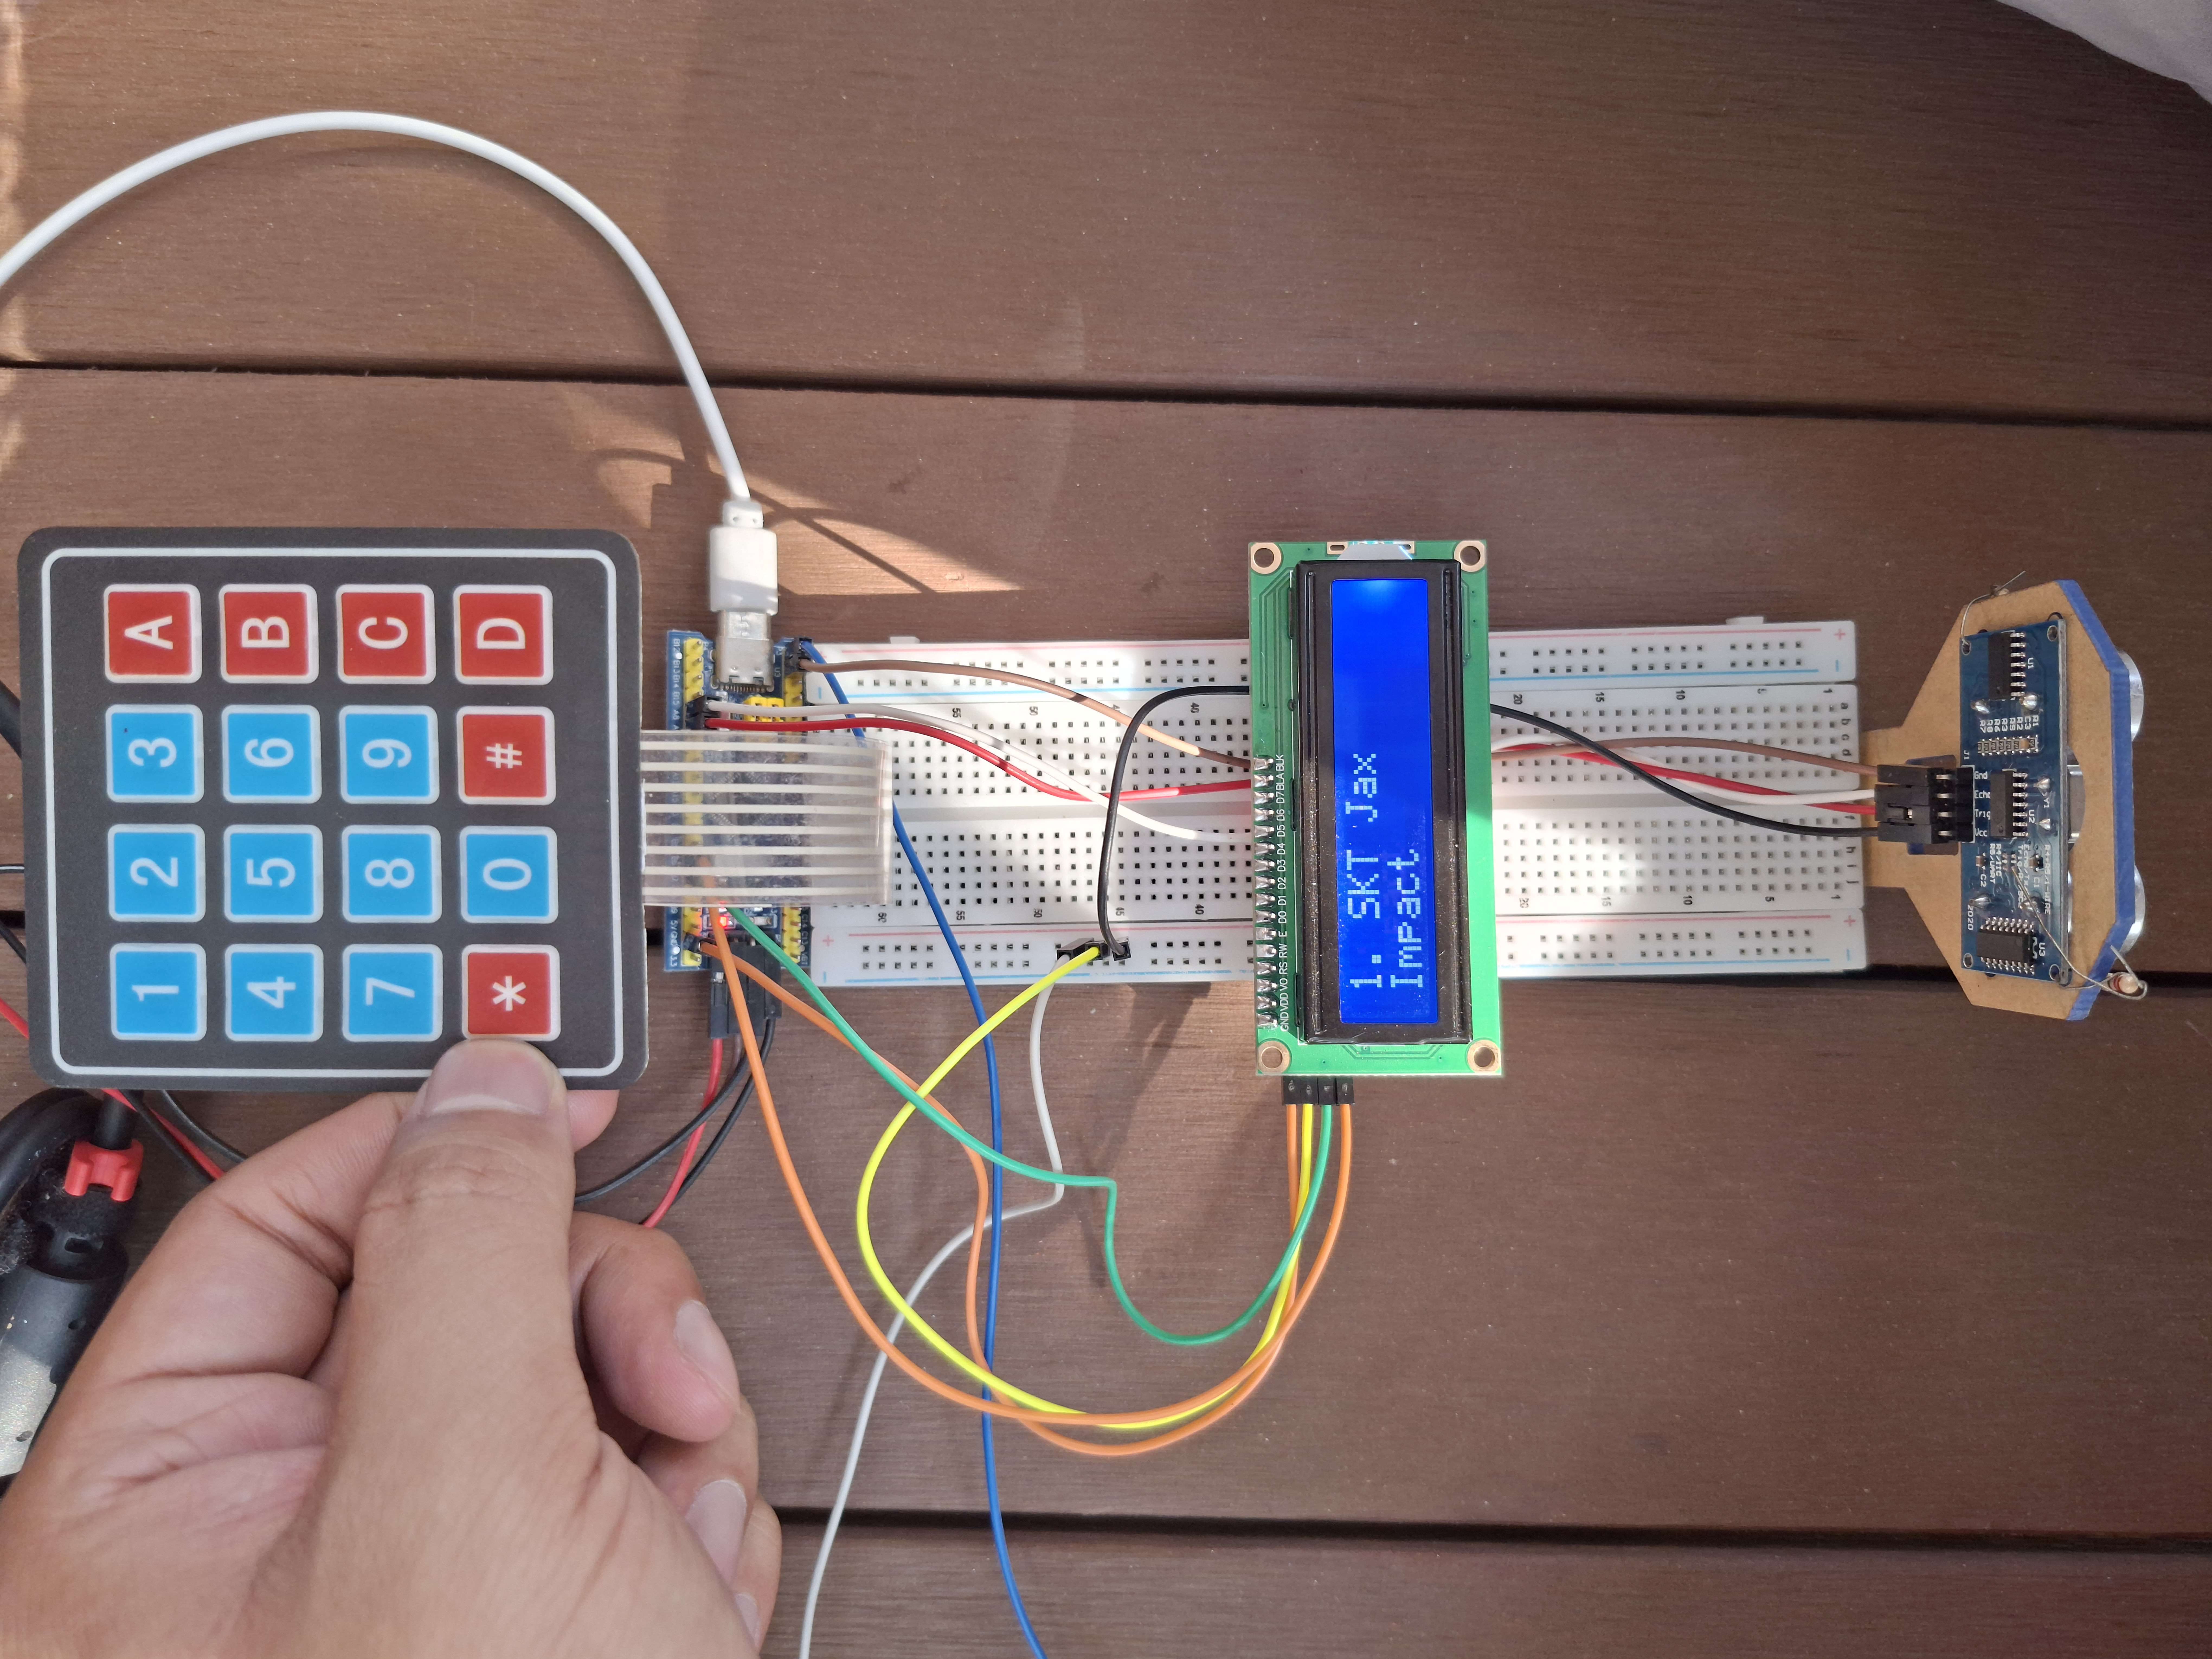
\includegraphics[width=0.9\textwidth]{../Pictures/topView.jpg}
    \caption{Hiện thực phần cứng của hệ thống Máy bán hàng tự động}
    \label{fig:hardware_overview}
\end{figure}

\subsection{Vi điều khiển - STM32F103C8T6}

STM32F103C8T6 (thường được gọi là "Blue Pill") đóng vai trò là đơn vị xử lý trung tâm của hệ thống.

STM32F103C8T6 được chọn vì:

\begin{itemize}[leftmargin=*]
    \item \textbf{Sức mạnh:} Xung nhịp 72 MHz cung cấp đủ hiệu năng cho các hoạt động thời gian thực
    \item \textbf{Bộ nhớ:} 64 KB Flash chứa được các trình điều khiển HAL và mã ứng dụng; 20 KB RAM đủ cho dữ liệu thời gian chạy
    \item \textbf{Hỗ trợ Ngoại vi:} Tích hợp sẵn I2C, timer và GPIO đáp ứng mọi yêu cầu giao diện
    \item \textbf{Thư viện đầy đủ:} Hỗ trợ tuyệt vời thông qua STM32CubeIDE và thư viện HAL
    \item \textbf{Chi phí:} Bo mạch giá rẻ có sẵn ở nhiều nơi.
    \item \textbf{Cộng đồng:} Cộng đồng người dùng lớn và tài liệu tham khảo/diễn đàn phong phú
\end{itemize}

Các pin quan trọng cho dự án này:

\begin{table}[H]
\centering
\caption{Gán chân STM32F103C8T6}
\begin{tabular}{|l|l|l|}
\hline
\textbf{Chân} & \textbf{Chức năng} & \textbf{Mô tả} \\
\hline
PA0-PA3 & Hàng Bàn phím & Chân đầu ra để quét bàn phím \\
PA4-PA7 & Cột Bàn phím & Chân đầu vào với điện trở pull-up \\
PB6 & I2C1\_SCL & Xung nhịp I2C cho giao tiếp LCD \\
PB7 & I2C1\_SDA & Dữ liệu I2C cho giao tiếp LCD \\
PA8 & TIM1\_CH1 & ECHO cảm biến siêu âm (Bắt đầu vào) \\
PA9 & GPIO Output & TRIG cảm biến siêu âm \\
PC13 & GPIO Output & Đèn báo LED (low-active) \\
PA13 & SWDIO & Dữ liệu I/O debug Serial Wire \\
PA14 & SWCLK & Xung nhịp debug Serial Wire \\
\hline
\end{tabular}
\end{table}

\subsection{LCD 1602 với I2C}

Hệ thống sử dụng màn hình LCD 16x2 kết hợp với bộ mở rộng I/O I2C PCF8574 để hiển thị thông tin.

Hệ thống hiện thực giao tiếp I2C bit-banged:

\begin{enumerate}[leftmargin=*]
    \item \textbf{Điều kiện START:} SDA chuyển từ cao xuống thấp trong khi SCL ở mức cao
    \item \textbf{Khung Địa chỉ:} Gửi địa chỉ slave 7-bit + bit R/W
    \item \textbf{Truyền Dữ liệu:} Gửi dữ liệu 8-bit với kiểm tra ACK
    \item \textbf{Điều kiện STOP:} SDA chuyển từ thấp lên cao trong khi SCL ở mức cao
\end{enumerate}

Đối với hoạt động LCD ở chế độ 4-bit:
\begin{enumerate}[leftmargin=*]
    \item Gửi nibble cao (4 bit) của byte dữ liệu
    \item Tạo xung chân Enable
    \item Gửi nibble thấp (4 bit) của byte dữ liệu
    \item Tạo xung chân Enable
\end{enumerate}

\subsection{Bàn phím Ma trận 4×4}

Bàn phím ma trận cung cấp 16 phím được sắp xếp thành 4 hàng và 4 cột, hoạt động dựa trên nguyên tắc quét hàng-cột.

Các công tắc cơ học như bàn phím này có hiện tượng nhiễu khi nhấn phím, gây ra nhiều input trong một lần nhấn. Hệ thống sẽ cần phải debouncing bằng phần mềm:

\begin{lstlisting}[language=C, caption={Hiện thực Chống bounce Bàn phím}]
if (HAL_GPIO_ReadPin(GPIOA, col_pins[c]) == GPIO_PIN_RESET) {
    HAL_Delay(20); // Debounce delay
    
    if (HAL_GPIO_ReadPin(GPIOA, col_pins[c]) == GPIO_PIN_RESET) {
        // Key press confirmed
        while (HAL_GPIO_ReadPin(GPIOA, col_pins[c]) == GPIO_PIN_RESET);
        // Wait for release
        return keymap[r][c];
    }
}
\end{lstlisting}

\subsection{Cảm biến Siêu âm HC-SR04}

HC-SR04 sử dụng phép đo time-of-flight để đo khoảng cách.

Hệ thống sử dụng Kênh 1 của TIM1 được cấu hình cho chế độ Input Capture:

\begin{itemize}[leftmargin=*]
    \item \textbf{Input Capture:} Cả hai cạnh (lên và xuống)
    \item \textbf{Tần số:} 1 MHz
    \item \textbf{Ngắt:} Được kích hoạt khi có tín hiệu Input Capture
\end{itemize}

\subsection{Bộ nhớ Flash}

Hệ thống sử dụng page cuối (page 63) của bộ nhớ Flash nội bộ để lưu trữ dữ liệu kho hàng, đảm bảo dữ liệu được bảo toàn khi mất điện.

Cấu trúc dữ liệu kho hàng (44 byte mỗi sản phẩm):
\begin{itemize}[leftmargin=*]
    \item \textbf{Magic number:} 4 byte (0xDEADBEEF)
    \item \textbf{Array sản phẩm:} 16 sản phẩm × 44 bytes = 704 bytes
    \item \textbf{Tổng:} 708 bytes (vừa khít trong 1KB của page Flash)
\end{itemize}

Khi bật nguồn:
\begin{enumerate}[leftmargin=*]
    \item Đọc số magic từ page 63 của Flash
    \item Nếu số magic khớp 0xDEADBEEF: Tải kho hàng từ Flash
    \item Nếu số magic invalid: Khởi tạo kho hàng mặc định và lưu vào Flash
\end{enumerate}


\section{Phần mềm}

\subsection{Máy trạng thái Hữu hạn}

\paragraph{Trạng thái Khởi tạo (1-2):}
\begin{itemize}[leftmargin=*]
    \item \textbf{INIT:} Khởi tạo hệ thống, thiết lập ngoại vi, tải kho hàng từ Flash
    \item \textbf{WAIT\_SENSOR:} trạng thái chờ với giám sát cảm biến siêu âm liên tục để phát hiện người dùng
\end{itemize}

\paragraph{Chế độ người dùng (3-14):}
\begin{itemize}[leftmargin=*]
    \item \textbf{WELCOME\_SECTION:} Hiển thị thông báo chào mừng trong 3 giây
    \item \textbf{CHOOSING\_SKIN:} Duyệt sản phẩm với điều hướng Lên/Xuống
    \item \textbf{DISPLAY\_INFO:} Hiển thị thông tin chi tiết sản phẩm (số lượng, giá)
    \item \textbf{CHOOSING\_QUANTITY:} Nhập số lượng (1-9)
    \item \textbf{OUT\_OF\_STOCK\_NOTIFICATION:} Cảnh báo khi sản phẩm đã chọn không có sẵn
    \item \textbf{QUANTITY\_ERROR:} Yêu cầu thử lại khi số lượng nhập vào không hợp lệ
    \item \textbf{MAX\_ERROR\_STATE:} Hủy giao dịch sau 5 lần lỗi liên tiếp
    \item \textbf{PAYMENT\_SHOW\_TOTAL:} Hiển thị tổng số tiền phải trả
    \item \textbf{PAYMENT\_INPUT:} Chỉ chấp nhận các mệnh giá thanh toán đã định (5K, 10K,..., 500K VND)
    \item \textbf{PAYMENT\_ERROR:} Yêu cầu thử lại khi mệnh giá không hợp lệ
    \item \textbf{PAYMENT\_INFO\_WAIT:} Hiển thị số tiền còn lại hoặc tiền thừa
    \item \textbf{THANKS:} Hiển thị màn hình THANKS và quay lại chọn sản phẩm
\end{itemize}

\paragraph{Chế độ Quản trị (15-19):}
\begin{itemize}[leftmargin=*]
    \item \textbf{ADMIN\_MODE:} Xác nhận đăng nhập thành công
    \item \textbf{CHOOSING\_SKIN\_TO\_ADJUST:} Chọn sản phẩm để config
    \item \textbf{TIMEOUT\_ADMIN\_MODE:} Tự động đăng xuất sau 60 giây không có tương tác
    \item \textbf{ADJUST\_QUANTITY\_AND\_PRICE:} Chỉnh sửa kho hàng và giá cả
    \item \textbf{CONFIRM\_EXIT\_ADMIN\_MODE:} Hộp thoại xác nhận đăng xuất YES NO
\end{itemize}

\textbf{Sơ đồ Chuyển đổi Trạng thái}

Các chuyển đổi trạng thái tuân theo các đường dẫn chính sau:

\begin{figure}[H]
    \centering
    \includegraphics[width=0.9\textwidth]{../Pictures/fsm.png}
    \caption{Sơ đồ chuyển đổi trạng thái (Chế độ Người dùng)}
    \label{fig:fsm_diagram}
\end{figure}

\begin{figure}[H]
    \centering
    \includegraphics[width=0.9\textwidth]{../Pictures/fsmAdmin.png}
    \caption{Sơ đồ chuyển đổi trạng thái (Chế độ Quản trị)}
    \label{fig:fsm_admin_diagram}
\end{figure}

\textbf{Luồng Giao dịch Bình thường:}
\begin{verbatim}
INIT -> WAIT_SENSOR -> WELCOME_SECTION -> CHOOSING_SKIN 
    -> DISPLAY_INFO -> CHOOSING_QUANTITY -> PAYMENT_SHOW_TOTAL 
    -> PAYMENT_INPUT -> PAYMENT_INFO_WAIT -> THANKS -> CHOOSING_SKIN
\end{verbatim}

\textbf{Xử lý Lỗi:}
\begin{itemize}[leftmargin=*]
    \item Lỗi số lượng: CHOOSING\_QUANTITY $\rightarrow$ QUANTITY\_ERROR $\rightarrow$ CHOOSING\_QUANTITY (hoặc MAX\_ERROR\_STATE sau 5 lần thử)
    \item Lỗi thanh toán: PAYMENT\_INPUT $\rightarrow$ PAYMENT\_ERROR $\rightarrow$ PAYMENT\_INPUT (hoặc INIT sau 5 lần thử)
    \item Hết hàng: DISPLAY\_INFO $\rightarrow$ OUT\_OF\_STOCK\_NOTIFICATION $\rightarrow$ DISPLAY\_INFO
    \item Thời gian chờ: Bất kỳ trạng thái người dùng nào $\rightarrow$ trạng thái phục hồi thích hợp sau 30 giây
\end{itemize}

\textbf{Login vào Chế độ Quản trị:}

Mật khẩu là: 070596

\begin{verbatim}
CHOOSING_SKIN (Phím D + mật khẩu) -> ADMIN_MODE 
    -> CHOOSING_SKIN_TO_ADJUST -> ADJUST_QUANTITY_AND_PRICE 
    -> CHOOSING_SKIN_TO_ADJUST hoặc CONFIRM_EXIT_ADMIN_MODE
\end{verbatim}

\subsection{Timer/Scheduler}

Hệ thống sử dụng cơ chế timer phần mềm để quản lý delay, thời gian chờ và chuyển đổi trạng thái mà không ngắt luồng thực thi.

\textbf{Các loại timer}

Năm loại timer độc lập được hiện thực:

\begin{table}[H]
\centering
\caption{Các loại timer Phần mềm}
\begin{tabular}{|l|l|p{6cm}|}
\hline
\textbf{Timer} & \textbf{Thời lượng} & \textbf{Mục đích} \\
\hline
init\_timer & 1000ms & Delay khởi tạo trước khi kích hoạt cảm biến \\
\hline
welcome\_timer & 3000ms & Thời gian hiển thị màn hình chào mừng \\
\hline
timeout\_timer & 30s / 60s & Thời gian chờ không hoạt động (user/admin) \\
\hline
message\_timer & 3000ms & Thời gian hiển thị thông báo (vd màn hình THANKS) \\
\hline
sensor\_timer & 100ms & Khoảng thời gian refresh cảm biến siêu âm \\
\hline
\end{tabular}
\end{table}

\textbf{Hiện thực timer}

Mỗi timer bao gồm ba thành phần:

\begin{lstlisting}[language=C, caption={Cấu trúc Dữ liệu timer}]
// Counter: Decremented each millisecond
int welcome_timer_counter = 0;

// Flag: Set to 1 when counter reaches 0
int welcome_timer_flag = 0;

// Setter function: Initialize counter and clear flag
void setWelcomeTimer(int duration) {
    welcome_timer_counter = duration;
    welcome_timer_flag = 0;
}
\end{lstlisting}

\textbf{Thực thi timer}

Hàm \texttt{timerRun()} được gọi mỗi 1ms (thường trong ngắt SysTick):

\begin{lstlisting}[language=C, caption={Hàm Cập nhật timer}]
void timerRun() {
    if (welcome_timer_counter > 0) {
        welcome_timer_counter--;
        if (welcome_timer_counter <= 0) {
            welcome_timer_flag = 1;
        }
    }
    // ... repeat for other timers ...
}
\end{lstlisting}

\textbf{Mẫu Sử dụng timer}

Cách sử dụng điển hình trong các trạng thái FSM:

\begin{lstlisting}[language=C, caption={Ví dụ Sử dụng timer}]
case WELCOME_SECTION:
    // State entry: Set timer
    if (entered_state) {
        setWelcomeTimer(3000);  // 3 second display
        lcd_clear();
        lcd_write_string("WELCOME!");
    }
    
    // State execution: Check flag
    if (welcome_timer_flag == 1) {
        status = CHOOSING_SKIN;  // Transition
        lcd_clear();
    }
    break;
\end{lstlisting}

\subsection{Cấu trúc Dữ liệu và Quản lý Bộ nhớ}

\textbf{Cấu trúc Dữ liệu Sản phẩm}

Hệ thống kho hàng sử dụng kiểu dữ liệu có cấu trúc cho sản phẩm:

\begin{lstlisting}[language=C, caption={Cấu trúc Dữ liệu Sản phẩm}]
typedef struct {
    uint8_t id;              // Product ID (1-16)
    char skinName[16];       // Product name (e.g., "SKT Jax")
    char playerName[16];     // Player name (e.g., "Impact")
    uint32_t quantity;       // Stock level (0-9)
    uint32_t price;          // Price in VND
} Skin;

// Global inventory array
Skin skt_skins[16];
\end{lstlisting}

44 byte mỗi sản phẩm × 16 sản phẩm = 704 byte

\textbf{Bố cục Bộ nhớ Flash}

Lưu trữ dữ liệu bằng bộ nhớ Flash nội bộ:

\begin{lstlisting}[language=C, caption={Cấu hình Bộ nhớ Flash}]
// Page 63 address: Last 1KB of 64KB Flash
#define FLASH_ADDR_PAGE_63  0x0800FC00

// Magic number for data validation
#define MAGIC_NUMBER        0xDEADBEEF

// Memory layout:
// Offset 0x00: Magic number (4 bytes)
// Offset 0x04: Skin array (704 bytes)
// Total: 708 bytes
\end{lstlisting}

\textbf{Biến Toàn cục}

Các variable trạng thái chính được duy trì bởi FSM:

\begin{lstlisting}[language=C, caption={Biến Trạng thái Toàn cục}]
int status = INIT;                    // Current FSM state
uint8_t current_id = 1;               // Selected product ID
uint32_t input_quantity = 0;          // User-entered quantity
uint8_t error_count = 0;              // Consecutive error counter

uint32_t total_payable = 0;           // Total payment required
uint32_t money_inserted_current = 0;  // Current denomination input
uint32_t money_paid_accumulated = 0;  // Total paid so far
uint8_t payment_error_count = 0;      // Payment error counter

uint32_t detection_start_time = 0;    // Sensor detection timestamp
\end{lstlisting}

\subsection{Các Thuật toán Chính}

\subsubsection{Thuật toán Phát hiện người dùng}

Hệ thống giám sát liên tục cảm biến siêu âm mỗi 100ms. Nếu phát hiện vật thể trong phạm vi 20cm trong 3 giây liên tiếp, hệ thống sẽ chuyển sang trạng thái chào mừng. Cơ chế này giúp lọc nhiễu và đảm bảo sự hiện diện có chủ ý của người dùng.

\subsubsection{Thuật toán để Thanh toán}

Thanh toán chỉ với các mệnh giá đã được chỉ định, không chấp nhận các mệnh giá khác:

\begin{lstlisting}[language=C, caption={Xác thực Thanh toán}]
// Valid Vietnamese currency denominations
int is_valid_money(uint32_t amount) {
    switch(amount) {
        case 5000:
        case 10000:
        case 20000:
        case 50000:
        case 100000:
        case 200000:
        case 500000:
            return 1;
        default:
            return 0;
    }
}

// Payment processing
if (is_valid_money(money_inserted_current)) {
    money_paid_accumulated += money_inserted_current;
    
    if (money_paid_accumulated < total_payable) {
        uint32_t remaining = total_payable - money_paid_accumulated;
        // Display remaining amount
    } else {
        uint32_t change = money_paid_accumulated - total_payable;
        // Payment complete, display change
        status = THANKS;
    }
} else {
    payment_error_count++;
    if (payment_error_count >= 5) {
        status = INIT;  // Abort transaction
    } else {
        status = PAYMENT_ERROR;  // Retry
    }
}
\end{lstlisting}

\subsubsection{Thuật toán Lưu trữ Kho hàng}

Đọc/ghi Flash có kiểm tra magic number:

\begin{lstlisting}[language=C, caption={Các hoạt động Bộ nhớ Flash}]
void Store_SaveToFlash(void) {
    // 1. Unlock Flash
    HAL_FLASH_Unlock();
    
    // 2. Erase page
    FLASH_EraseInitTypeDef EraseInitStruct;
    uint32_t PageError;
    EraseInitStruct.TypeErase = FLASH_TYPEERASE_PAGES;
    EraseInitStruct.PageAddress = FLASH_ADDR_PAGE_63;
    EraseInitStruct.NbPages = 1;
    HAL_FLASHEx_Erase(&EraseInitStruct, &PageError);
    
    // 3. Write magic number
    HAL_FLASH_Program(FLASH_TYPEPROGRAM_WORD, 
                      FLASH_ADDR_PAGE_63, 
                      MAGIC_NUMBER);
    
    // 4. Write data array
    uint32_t *pData = (uint32_t*)skt_skins;
    uint32_t numWords = sizeof(skt_skins) / 4;
    
    for (uint32_t i = 0; i < numWords; i++) {
        uint32_t address = FLASH_ADDR_PAGE_63 + 4 + (i * 4);
        HAL_FLASH_Program(FLASH_TYPEPROGRAM_WORD, address, pData[i]);
    }
    
    // 5. Lock Flash
    HAL_FLASH_Lock();
}

void init(void) {
    uint32_t stored_magic = *(__IO uint32_t*)FLASH_ADDR_PAGE_63;
    
    if (stored_magic == MAGIC_NUMBER) {
        // Valid data exists: Load from Flash
        uint32_t *pFlashData = (uint32_t*)(FLASH_ADDR_PAGE_63 + 4);
        uint32_t *pRamData = (uint32_t*)skt_skins;
        uint32_t numWords = sizeof(skt_skins) / 4;
        
        for (uint32_t i = 0; i < numWords; i++) {
            pRamData[i] = pFlashData[i];
        }
    } else {
        // First boot: Initialize defaults
        skt_skins[0] = (Skin){1, "SKT Jax", "Impact", 9, 20000};
        // ... initialize 15 more products ...
        Store_SaveToFlash();
    }
}
\end{lstlisting}

\subsubsection{Thuật toán Xác thực Quản trị}

Xác minh mật khẩu với thời gian chờ:

\begin{lstlisting}[language=C, caption={Xác minh Mật khẩu Quản trị}]
const char password[] = "070596";
#define MAX_INPUT 6

int admin_log(void) {
    char input[MAX_INPUT + 1] = {0};
    int len = 0;
    uint32_t last_tick = HAL_GetTick();
    
    lcd_clear();
    lcd_write_string("ENTER PASSWORD");
    
    while (1) {
        // 10-second timeout
        if (HAL_GetTick() - last_tick > 10000) {
            return 0;  // Timeout
        }
        
        char c = Keypad_Scan();
        if (c == 0) continue;
        
        last_tick = HAL_GetTick();  // Reset timeout
        
        if (c >= '0' && c <= '9') {
            if (len < MAX_INPUT) {
                input[len++] = c;
                lcd_write_char('*');  // Masked display
                
                if (len == MAX_INPUT) {
                    HAL_Delay(200);
                    return (strcmp(password, input) == 0) ? 1 : 0;
                }
            }
        } else if (c == '*') {  // Backspace
            if (len > 0) {
                len--;
                input[len] = '\0';
                // Clear last asterisk
            } else {
                return 0;  // Quick exit
            }
        }
        
        HAL_Delay(100);  // Debouncing
    }
}
\end{lstlisting}

\subsection{Project Structure}

\paragraph{Cấu trúc module:}

Dự án có source code tuân theo kiến trúc module với sự phân tách rõ ràng:

\begin{table}[H]
\centering
\caption{Các module Phần mềm}
\begin{tabular}{|l|p{10cm}|}
\hline
\textbf{module} & \textbf{Nhiệm vụ} \\
\hline
main.c & File chính của chương trình, khởi tạo ngoại vi, vòng lặp chính \\
\hline
fsm\_vm.c/h & Logic máy trạng thái hữu hạn, chuyển đổi trạng thái\\
\hline
store.c/h & Quản lý dữ liệu kho hàng, đọc/ghi Flash \\
\hline
keypad.c/h & Quét bàn phím ma trận, có debouncing, ánh xạ ký tự nhập vào màn hình\\
\hline
sensor.c/h & Kích hoạt cảm biến siêu âm, đo khoảng cách \\
\hline
tv\_lcd\_i2c.c/h & Điều khiển hiển thị LCD, giao tiếp I2C, định dạng văn bản \\
\hline
i2c.c/h & Giao thức I2C \\
\hline
timer.c/h & Quản lý soft-timer, xử lý thời gian chờ \\
\hline
ADMIN.c/h & Xác thực admin, xác minh mật khẩu \\
\hline
\end{tabular}
\end{table}

\paragraph{Module Hierarchy:}

Phân cấp phụ thuộc (từ trên xuống dưới):
\begin{verbatim}
main.c
  - fsm_vm.c
    - store.c (Flash operations)
    - keypad.c (user input)
    - sensor.c (customer detection)
    - tv_lcd_i2c.c (display)
        - i2c.c (communication protocol)
        - timer.c (timeouts)
    - ADMIN.c (authentication)
\end{verbatim}

\section{Hiện thực}

\subsection{Hiện thực Trình điều khiển Ngoại vi}

\paragraph{Trình điều khiển LCD I2C:}

Trình điều khiển LCD được hiện thực chế độ giao tiếp 4-bit 
thông qua giao thức I2C bit-banged. 
Cách tiếp cận này đảm bảo tương thích 
với các bo mạch chuyển đổi PCF8574 khác nhau và có khả năng kiểm soát 
thời gian tốt hơn.

\paragraph{Các hàm Giao thức I2C:}

.

\begin{lstlisting}[language=C, caption={Hiện thực I2C Bit-Banged}]
void I2C_Start(void) {
    // START condition: SDA high to low while SCL high
    HAL_GPIO_WritePin(I2C_SDA_PORT, I2C_SDA_PIN, GPIO_PIN_SET);
    HAL_GPIO_WritePin(I2C_SCL_PORT, I2C_SCL_PIN, GPIO_PIN_SET);
    delay_us(5);
    HAL_GPIO_WritePin(I2C_SDA_PORT, I2C_SDA_PIN, GPIO_PIN_RESET);
    delay_us(5);
    HAL_GPIO_WritePin(I2C_SCL_PORT, I2C_SCL_PIN, GPIO_PIN_RESET);
}

void I2C_Write(uint8_t data) {
    for (int i = 0; i < 8; i++) {
        // Write MSB first
        if (data & 0x80) {
            HAL_GPIO_WritePin(I2C_SDA_PORT, I2C_SDA_PIN, GPIO_PIN_SET);
        } else {
            HAL_GPIO_WritePin(I2C_SDA_PORT, I2C_SDA_PIN, GPIO_PIN_RESET);
        }
        delay_us(5);
        HAL_GPIO_WritePin(I2C_SCL_PORT, I2C_SCL_PIN, GPIO_PIN_SET);
        delay_us(5);
        HAL_GPIO_WritePin(I2C_SCL_PORT, I2C_SCL_PIN, GPIO_PIN_RESET);
        data <<= 1;
    }
}
\end{lstlisting}

\paragraph{Các hàm Chế độ LCD 4-Bit:}

.

\begin{lstlisting}[language=C, caption={Các hàm Giao tiếp LCD}]
void LCD_Send4Bit(unsigned char Data) {
    data_MASK &= 0x0F;  // Clear upper 4 bits
    // Map data bits to PCF8574 pins P4-P7
    data_MASK |= (Data & 0x01) << 4;
    data_MASK |= (Data & 0x02) << 4;
    data_MASK |= (Data & 0x04) << 4;
    data_MASK |= (Data & 0x08) << 4;
}

void LCD_Send1Byte(unsigned char byte) {
    LCD_Send4Bit(byte >> 4);  // Send upper nibble
    LCD_Enable();              // Pulse enable
    LCD_Send4Bit(byte);        // Send lower nibble
    LCD_Enable();              // Pulse enable
}

void LCD_Enable(void) {
    data_MASK |= LCD_EN;       // Set enable bit
    for(int i=0; i<50; i++) __NOP();
    PCD8574_write(data_MASK);
    data_MASK &= ~LCD_EN;      // Clear enable bit
    for(int i=0; i<100; i++) __NOP();
    PCD8574_write(data_MASK);
}
\end{lstlisting}

\paragraph{Trình tự Khởi tạo LCD:}

.

\begin{lstlisting}[language=C, caption={Khởi tạo LCD}]
void lcd_init(uint8_t addr) {
    LCDI2C_ADDR = addr;
    
    // Power-on delay
    HAL_Delay(50);
    
    // 8-bit mode initialization sequence
    LCD_Send4Bit(0x03);
    LCD_Enable();
    HAL_Delay(5);
    LCD_Enable();
    HAL_Delay(5);
    LCD_Enable();
    
    // Switch to 4-bit mode
    LCD_Send4Bit(0x02);
    LCD_Enable();
    
    // Function set: 4-bit, 2 lines, 5x8 font
    LCD_Send1Byte(0x28);
    
    // Display control: Display on, cursor off
    LCD_Send1Byte(0x0C);
    
    // Entry mode: Increment cursor, no shift
    LCD_Send1Byte(0x06);
    
    lcd_clear();
}
\end{lstlisting}

\paragraph{Trình điều khiển Bàn phím}

Trình điều khiển bàn phím hiện thực quét hàng với debouncing:

\begin{lstlisting}[language=C, caption={Hiện thực Scan Bàn phím}]
char Keypad_Scan(void) {
    // Key mapping array
    static const char keymap[4][4] = {
        {'1','2','3','U'},
        {'4','5','6','D'},
        {'7','8','9','L'},
        {'*','0','#','R'}
    };
    
    for (int r = 0; r < 4; r++) {
        // Set all rows HIGH
        HAL_GPIO_WritePin(GPIOA, 
                          GPIO_PIN_0 | GPIO_PIN_1 | 
                          GPIO_PIN_2 | GPIO_PIN_3,
                          GPIO_PIN_SET);
        
        // Pull current row LOW
        HAL_GPIO_WritePin(GPIOA, row_pins[r], GPIO_PIN_RESET);
        HAL_Delay(1);
        
        // Read all columns
        for (int c = 0; c < 4; c++) {
            if (HAL_GPIO_ReadPin(GPIOA, col_pins[c]) == GPIO_PIN_RESET) {
                // Key pressed detected
                HAL_Delay(20);  // Debounce delay
                
                // Confirm key still pressed
                if (HAL_GPIO_ReadPin(GPIOA, col_pins[c]) == GPIO_PIN_RESET) {
                    // Wait for key release
                    while (HAL_GPIO_ReadPin(GPIOA, col_pins[c]) 
                           == GPIO_PIN_RESET);
                    
                    return keymap[r][c];
                }
            }
        }
    }
    return 0;  // No key pressed
}
\end{lstlisting}

\paragraph{Trình điều khiển Cảm biến Siêu âm}

Trình điều khiển cảm biến sử dụng timer bắt tín hiệu đầu vào 
để đo thời gian phản hồi của xung siêu âm. 
Quá trình đo bao gồm kích hoạt xung Trigger và 
đo độ rộng xung Echo sử dụng ngắt Input Capture.

\begin{lstlisting}[language=C, caption={Đo khoảng cách với HC-SR04}]
void Sensor_Trigger(void) {
    HAL_GPIO_WritePin(TRIG_PORT, TRIG_PIN, GPIO_PIN_SET);
    delay_us(10);
    HAL_GPIO_WritePin(TRIG_PORT, TRIG_PIN, GPIO_PIN_RESET);
    __HAL_TIM_ENABLE_IT(&htim1, TIM_IT_CC1);
}

void HAL_TIM_IC_CaptureCallback(TIM_HandleTypeDef *htim) {
    if (htim->Channel == HAL_TIM_ACTIVE_CHANNEL_1) {
        if (Is_First_Captured==0) {
            IC_Val1 = HAL_TIM_ReadCapturedValue(htim, TIM_CHANNEL_1);
            Is_First_Captured = 1;
            __HAL_TIM_SET_CAPTUREPOLARITY(htim, TIM_CHANNEL_1, 
                                        TIM_INPUTCHANNELPOLARITY_FALLING);
        }
        else if (Is_First_Captured==1) {
            IC_Val2 = HAL_TIM_ReadCapturedValue(htim, TIM_CHANNEL_1);
            __HAL_TIM_SET_COUNTER(htim, 0);

            if (IC_Val2 > IC_Val1) 
                Difference = IC_Val2-IC_Val1;
            else 
                Difference = (0xffff - IC_Val1) + IC_Val2;

            Distance = Difference * .034/2;
            Is_First_Captured = 0;

            __HAL_TIM_SET_CAPTUREPOLARITY(htim, TIM_CHANNEL_1, 
                                        TIM_INPUTCHANNELPOLARITY_RISING);
            __HAL_TIM_DISABLE_IT(&htim1, TIM_IT_CC1);
        }
    }
}
\end{lstlisting}

\subsection{Hiện thực Máy trạng thái}

\textbf{Hiện thực các Trạng thái quan trọng:}

\paragraph{Trạng thái CHOOSING\_SKIN:}

.

\begin{lstlisting}[language=C, caption={Trạng thái CHOOSING\_SKIN}]
case CHOOSING_SKIN:
{
    if (timeout_timer_flag == 1) {
        status = INIT;
        fsm_init();
        break;
    }
    
    char key = Keypad_Scan();
    if (key != 0) {
        setTimeoutTimer(30000);  // Reset 30s timeout
        
        if (key == 'U') {
            current_id--;
            if (current_id < 1) current_id = 16;  // Wrap around
            display_current_skin(current_id);
        }
        else if (key == 'D') {
            current_id++;
            if (current_id > 16) current_id = 1;  // Wrap around
            display_current_skin(current_id);
        }
        else if (key == '#') {
            status = DISPLAY_INFO;
            lcd_clear();
            display_skin_detail(current_id);
        }
        else if (key == 'R') {
            int is_admin = admin_log();
            if (is_admin) {
                status = ADMIN_MODE;
                // Display admin success message
            }
        }
    }
}
break;
\end{lstlisting}

\paragraph{Trạng thái PAYMENT\_INPUT:}

Trạng thái này xử lý việc nhập tiền từ người dùng, 
cộng dồn số tiền đã insert và kiểm tra xem đã đủ để thanh toán chưa.

\begin{lstlisting}[language=C, caption={PAYMENT\_INPUT}]
case PAYMENT_INPUT:
{
    if (timeout_timer_flag == 1) {
        // Timeout handling...
        break;
    }

    char key = Keypad_Scan();
    if (key != 0) {
        setTimeoutTimer(30000);

        if (key >= '0' && key <= '9') {
            // Accumulate input amount
            if (money_inserted_current < 1000000000) {
                money_inserted_current = money_inserted_current * 10 + (key - '0');
                display_payment_input();
            }
        }
        else if (key == '#') {
            if (!is_valid_money(money_inserted_current)) {
                payment_error_count++;
                // Error handling...
            }
            else {
                money_paid_accumulated += money_inserted_current;

                if (money_paid_accumulated < total_payable) {
                    status = PAYMENT_INFO_WAIT;
                    // Show remaining amount
                }
                else {
                    status = PAYMENT_INFO_WAIT;
                    // Show change and success
                }
            }
        }
    }
}
break;
\end{lstlisting}

\paragraph{Trạng thái ADMIN\_MODE:}

Chế độ admin cho phép quản trị viên/người nhập kho thay đổi giá cả và tồn kho của từng sản phẩm.

\begin{lstlisting}[language=C, caption={Chế độ Quản trị}]
case CHOOSING_SKIN_TO_ADJUST:
{
    if (timeout_timer_flag == 1) {
        status = TIMEOUT_ADMIN_MODE;
        break;
    }

    char key = Keypad_Scan();
    if (key != 0) {
        setTimeoutTimer(60000);

        if (key == 'U') {
            current_id--;
            if (current_id < 1) current_id = 16;
            display_current_skin(current_id);
        }
        else if (key == 'D') {
            current_id++;
            if (current_id > 16) current_id = 1;
            display_current_skin(current_id);
        }
        else if (key == '#') {
            status = ADJUST_QUANTITY_AND_PRICE;
            lcd_clear();
            display_adjust_quantity_and_price(current_id, 0);
        }
    }
}
break;
\end{lstlisting
        if (key == 'U') {
            current_id--;
            if (current_id < 1) current_id = 16;  // Wrap around
            display_current_skin(current_id);
        }
        else if (key == 'D') {
            current_id++;
            if (current_id > 16) current_id = 1;  // Wrap around
            display_current_skin(current_id);
        }
        else if (key == '#') {
            status = DISPLAY_INFO;
            lcd_clear();
            display_skin_detail(current_id);
        }
        else if (key == 'R') {
            int is_admin = admin_log();
            if (is_admin) {
                status = ADMIN_MODE;
                // Display admin success message
            }
        }
    }
}
break;
\end{lstlisting}

\subsection{Giao diện hiển thị}

\paragraph{Các hàm hiển thị}

.

\begin{lstlisting}[language=C, caption={Các hàm hiển thị LCD}]
void lcd_center_text(int row, char *str) {
    int len = strlen(str);
    int padding = 0;
    if (len < 16) {
        padding = (16 - len) / 2;
    }
    lcd_gotoxy(padding, row);
    lcd_write_string(str);
}

void display_current_skin(uint8_t id) {
    Skin* skin = getSkinByID(id);
    if (skin == NULL) return;
    
    char buffer[22];
    
    // Line 1: ID and skin name
    lcd_gotoxy(0, 0);
    snprintf(buffer, sizeof(buffer), "%d. %-12s", 
             skin->id, skin->skinName);
    lcd_write_string(buffer);
    
    // Line 2: Player name
    lcd_gotoxy(0, 1);
    snprintf(buffer, sizeof(buffer), "%-16s", 
             skin->playerName);
    lcd_write_string(buffer);
}

void display_skin_detail(uint8_t id) {
    Skin* skin = getSkinByID(id);
    if (skin == NULL) return;
    
    char buffer[17];
    
    // Line 1: Available quantity
    lcd_gotoxy(0, 0);
    snprintf(buffer, sizeof(buffer), "Available: %-5lu", 
             (unsigned long)skin->quantity);
    lcd_write_string(buffer);
    
    // Line 2: Price and ID
    lcd_gotoxy(0, 1);
    snprintf(buffer, sizeof(buffer), "Price: %lu #%-3d", 
             (unsigned long)skin->price, skin->id);
    lcd_write_string(buffer);
}
\end{lstlisting}

\subsection{Cơ chế Xử lý Lỗi}

\paragraph{Kiểm tra INPUT}

.

\begin{lstlisting}[language=C, caption={Các hàm Kiểm tra INPUT}]
// Quantity validation
int validate_quantity(uint32_t quantity, uint32_t available) {
    if (quantity <= 0 || quantity > 9) {
        return ERROR_INVALID_RANGE;
    }
    if (quantity > available) {
        return ERROR_INSUFFICIENT_STOCK;
    }
    return VALIDATION_OK;
}

// Payment validation
int is_valid_money(uint32_t amount) {
    uint32_t valid_denominations[] = {
        5000, 10000, 20000, 50000, 
        100000, 200000, 500000
    };
    
    for (int i = 0; i < 7; i++) {
        if (amount == valid_denominations[i]) {
            return 1;
        }
    }
    return 0;
}
\end{lstlisting}

\paragraph{Số lần Lỗi Tối đa}

.

\begin{lstlisting}[language=C, caption={Không quá 5 lần Lỗi}]
// In CHOOSING_QUANTITY state
if (validation_error) {
    error_count++;
    
    if (error_count >= 5) {
        status = MAX_ERROR_STATE;
        lcd_clear();
        lcd_write_string("5 TIMES WRONG!");
        lcd_gotoxy(0, 1);
        lcd_write_string("DONT WANNA BUY?");
        setMessageTimer(3000);
    } else {
        status = QUANTITY_ERROR;
        // Display specific error message
        setMessageTimer(3000);
    }
}

// Reset counter on successful input
if (validation_success) {
    error_count = 0;
}
\end{lstlisting}

\subsection{Tối ưu hiệu năng}

\paragraph{Giảm số lần cập nhật hiển thị:}

Chỉ cập nhật LCD khi nội dung thay đổi:

\begin{lstlisting}[language=C, caption={Giảm số lần refresh LCD}]
static uint8_t last_displayed_id = 0;

void display_current_skin(uint8_t id) {
    if (id == last_displayed_id) {
        return;  // No change, skip update
    }
    
    last_displayed_id = id;
    // Perform actual display update
}
\end{lstlisting}

\paragraph{Tối ưu Timer:}

Chỉ sử dụng một SysTick duy nhất cho tất cả timer:

\begin{lstlisting}[language=C, caption={Tối ưu Quản lý Timer}]
void SysTick_Handler(void) {
    HAL_IncTick();
    timerRun();  // Update all software timers
}
\end{lstlisting}

\paragraph{Tối ưu khi ghi Flash:}

Chỉ ghi Flash khi dữ liệu thực sự thay đổi:

\begin{lstlisting}[language=C, caption={Tối ưu khi ghi Flash}]
int updateQuantity(uint8_t ID, uint32_t NEW_QUANTITY) {
    Skin* skin = getSkinByID(ID);
    if (skin == NULL || NEW_QUANTITY > 9) return 0;
    
    if (skin->quantity == NEW_QUANTITY) {
        return 1;  // No change, skip Flash write
    }
    
    skin->quantity = NEW_QUANTITY;
    Store_SaveToFlash();
    return 1;
}
\end{lstlisting}

\subsection{Phát triển và Debug}

\paragraph{Debug bằng UART:}

Để debug trong quá trình phát triển, có thể thêm giao tiếp UART:

\begin{lstlisting}[language=C, caption={Ví dụ Debug}]
#ifdef DEBUG_MODE
    printf("State: %d -> %d\n", old_status, status);
    printf("Distance: %d cm\n", Distance);
    printf("Key pressed: %c\n", key);
#endif
\end{lstlisting}

\paragraph{Giám sát Máy trạng thái với LED:}

Dùng một LED để chỉ báo trạng thái hệ thống:

\begin{lstlisting}[language=C, caption={Trạng thái LED}]
void update_status_led(void) {
    if (status == WAIT_SENSOR) {
        HAL_GPIO_WritePin(GPIOC, GPIO_PIN_13, GPIO_PIN_SET);  // Off
    } else {
        HAL_GPIO_WritePin(GPIOC, GPIO_PIN_13, GPIO_PIN_RESET); // On
    }
}
\end{lstlisting}


\section{Demo}

Phần này trình bày các quy trình kiểm thử, kết quả vận hành và 
phân tích hiệu năng của hệ thống máy bán hàng tự động.\newline
Xem thêm video trình diễn tại: \url{https://youtu.be/EFUxOFmGWq4?si=UAjL1COVcYWAQKlN}

\begin{figure}[H]
    \centering
    \begin{subfigure}[b]{0.45\textwidth}
        \centering
        \includegraphics[width=\textwidth]{../Pictures/quickDemo_1.png}
        \caption{Demo vận hành hệ thống}
        \label{fig:demo_1}
    \end{subfigure}
    \hfill
    \begin{subfigure}[b]{0.45\textwidth}
        \centering
        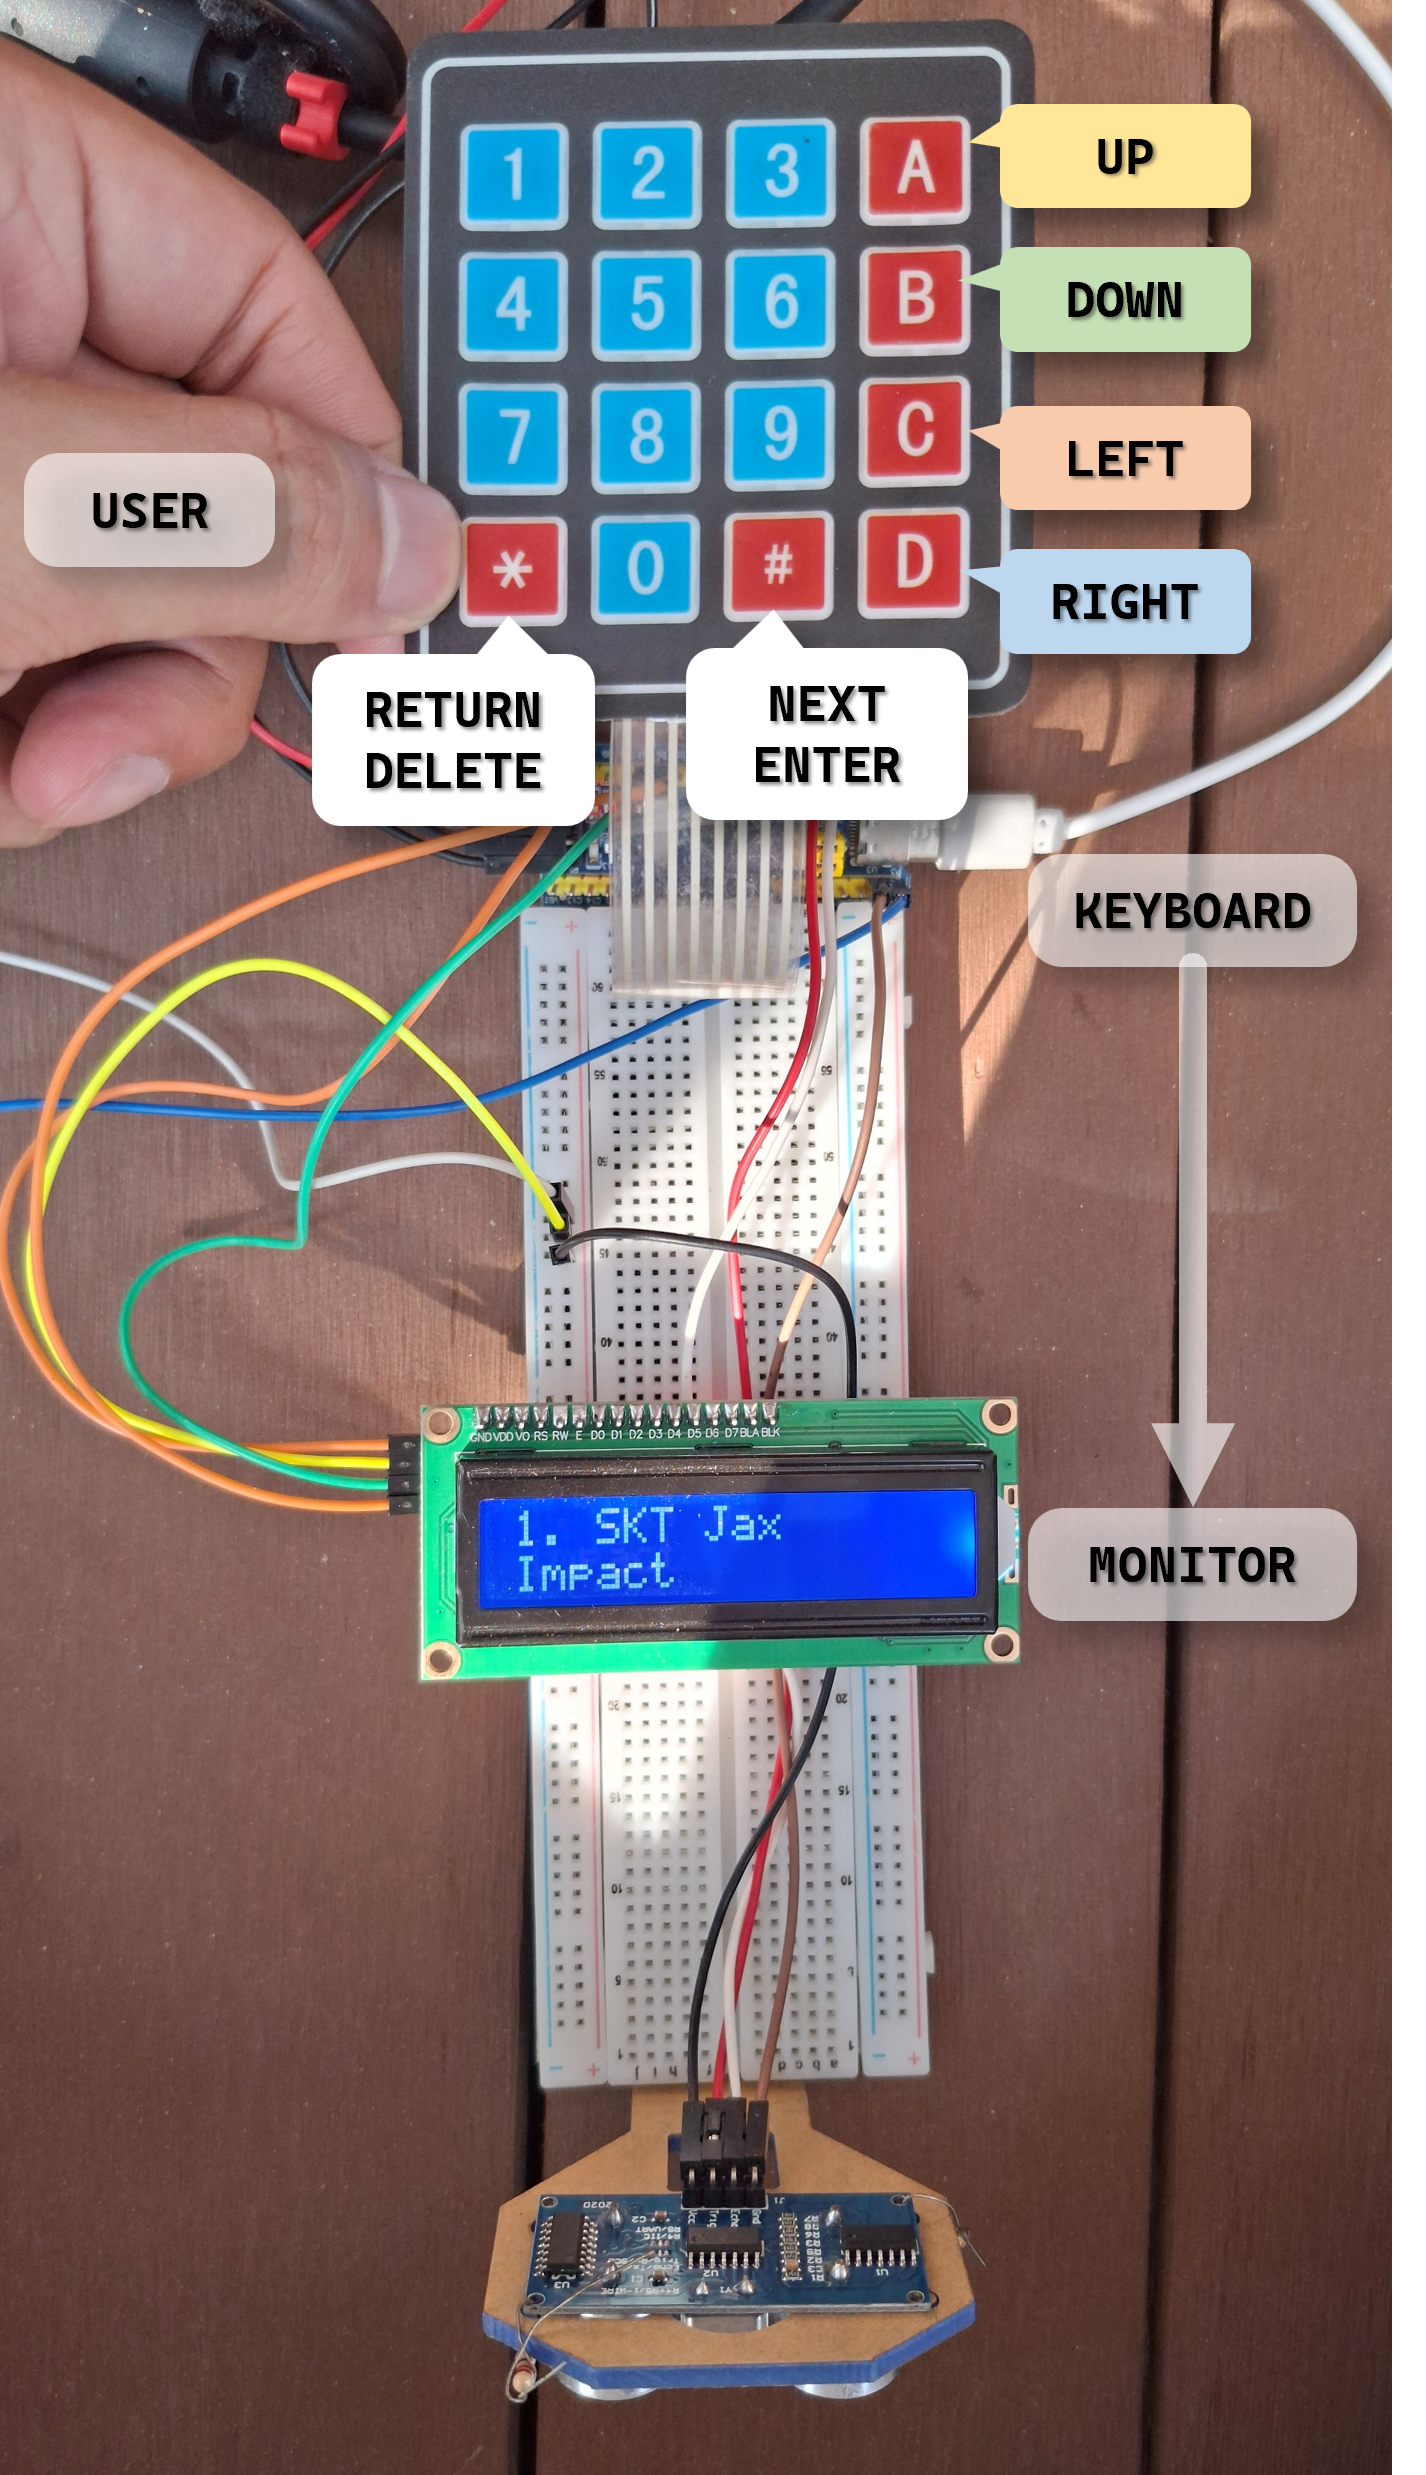
\includegraphics[width=\textwidth]{../Pictures/quickDemo_2.png}
        \caption{Demo vận hành hệ thống}
        \label{fig:demo_2}
    \end{subfigure}
    \caption{Demo vận hành Máy bán hàng tự động}
    \label{fig:system_demo}
\end{figure}

\textbf{Tất cả các input gây lỗi đã được test qua:}

\begin{itemize}[leftmargin=*]
    \item Đầu vào số lượng không hợp lệ bị từ chối và yêu cầu thử lại
    \item Số tiền thanh toán không hợp lệ kích hoạt thông báo lỗi và yêu cầu nhập lại
    \item Thống báo hết hàng và hướng dẫn người dùng chọn sản phẩm khác
    \item Hệ thống tự động hủy giao dịch sau 30 giây không hoạt động
    \item Chế độ quản trị tự động đăng xuất hoạt động chính xác sau 60 giây không hoạt động
    \item Lỗi quá 5 lần liên tiếp sẽ hủy giao dịch và trở về trạng thái ban đầu
\end{itemize}


\section{Kết luận}

\subsection{Thành tựu Dự án}

\begin{itemize}[leftmargin=*]
    \item \textbf{Tích hợp Phần cứng Hoàn chỉnh:} Giao tiếp thành công với màn hình LCD, bàn phím ma trận, cảm biến siêu âm và bộ nhớ Flash.
    
    \item \textbf{Hiện thực Máy trạng thái Mạnh mẽ:} Phát triển một FSM với nhiều trạng thái quản lý các luồng giao dịch phức tạp, xử lý lỗi và các chức năng quản trị.
    
    \item \textbf{Dữ liệu luôn được lưu lại:} Hiện thực lưu trữ tận dụng bộ nhớ Flash với magic number, đảm bảo dữ liệu kho hàng tồn tại dù bị mất điện.
    
    \item \textbf{Trình điều khiển Ngoại vi Tùy chỉnh:} Tạo các trình điều khiển hiệu quả cho giao tiếp LCD I2C bit-banged, quét bàn phím debouncing và đo khoảng cách.
    
    \item \textbf{Xử lý Lỗi hiệu quả:} Hiện thực kiểm tra đầu vào, quản lý timeout, bộ đếm lỗi và cơ chế thử lại đảm bảo độ sự thân thiện với người dùng.
    
    \item \textbf{Tự động Phát hiện người dùng:} Thành công bãi bỏ công tắc ON/OFF truyền thống, cung cấp trải nghiệm mới mẻ mà tiết kiệm điện năng.
    
    \item \textbf{Bảo mật tài khoản Quản trị:} Cung cấp chế độ quản trị được bảo vệ bằng mật khẩu với cơ chế tự đăng xuất kể cả khi quên.
\end{itemize}

\subsection{Ứng dụng Thực tế}

Mặc dù được phát triển như một dự án giáo dục, 
hệ thống thể hiện các khái niệm áp dụng cho máy bán hàng tự động 
thương mại và tự động hóa bán lẻ:

\begin{itemize}[leftmargin=*]
    \item Tự động phát hiện người dùng giảm tiêu thụ năng lượng
    \item Theo dõi kho hàng cho phép quản lí kinh doanh hiệu quả
    \item Xử lý lỗi cùng cơ chế thử lại nâng cao trải nghiệm người dùng
    \item Chế độ quản trị hỗ trợ bảo trì tại chỗ
    \item Thiết kế module tạo thuận lợi cho mở rộng tính năng
\end{itemize}

Kiến trúc có thể được thích ứng cho các kịch bản bán lẻ tự động 
khác nhau bao gồm máy bán hàng truyền thống, 
ki-ốt bán vé, hệ thống cho thuê và tủ khóa thông minh.


\section{Thông tin Dự án}

\subsection{GitHub repository}

Mã nguồn dự án, tài liệu và tài nguyên có sẵn tại:

\begin{itemize}[leftmargin=*]
    \item \textbf{GitHub:} \url{https://github.com/1172005thinh/VendingMachine}
    \item \textbf{Source code} Thư mục VendingMachine/ chứa tất cả các tệp nguồn
    \item \textbf{Tài liệu:} README.md với hướng dẫn thiết lập
\end{itemize}

\subsection{Tác giả}

\begin{table}[H]
\centering
\begin{tabular}{|l|p{8cm}|}
\hline
\textbf{Tên} & \textbf{Đóng góp} \\
\hline
\textbf{Nguyễn Hưng Thịnh} & 
\begin{itemize}[leftmargin=*, nosep, after=\strut]
    \item Tích hợp phần cứng và thiết kế mạch
    \item Kiểm thử và debug hệ thống
    \item Chuẩn bị tài liệu
    \item Quan lý dự án và phối hợp nhóm
    \item Quay video trình diễn và soạn thảo báo cáo cuối cùng
\end{itemize} \\
\hline
\textbf{Lê Thế Lộc} & 
\begin{itemize}[leftmargin=*, nosep, after=\strut]
    \item Phát triển trình điều khiển bàn phím
    \item Hệ thống quản lý kho hàng
    \item Các hoạt động bộ nhớ Flash
    \item Thiết kế kiến trúc hệ thống
    \item Phát triển trình điều khiển cảm biến
\end{itemize} \\
\hline
\textbf{Trần Doãn Hoàng Lâm} & 
\begin{itemize}[leftmargin=*, nosep, after=\strut]
    \item Thiết kế và hiện thực máy trạng thái hữu hạn
    \item Hiện thực hệ thống timer
    \item Thiết kế giao diện người dùng
    \item Thực hiện, soạn kịch bản trình diễn
\end{itemize} \\
\hline
\end{tabular}
\end{table}

\subsection{Lời cảm ơn}

Các tác giả xin bày tỏ lòng biết ơn đến:

\begin{itemize}[leftmargin=*]
    \item Thầy Nguyễn Thành Lộc đã hướng dẫn các nguyên tắc thiết kế hệ thống luận lý
    \item Cộng đồng mã nguồn mở về các ví dụ mã và hỗ trợ khắc phục sự cố
\end{itemize}

\end{document}
